\providecommand{\main}{../../../..}
\documentclass[\main/dresen_thesis.tex]{subfiles}

\begin{document}
  \label{sec:monolayers:magneticStructure:vsm}
  \begin{figure}[tb]
    \centering
    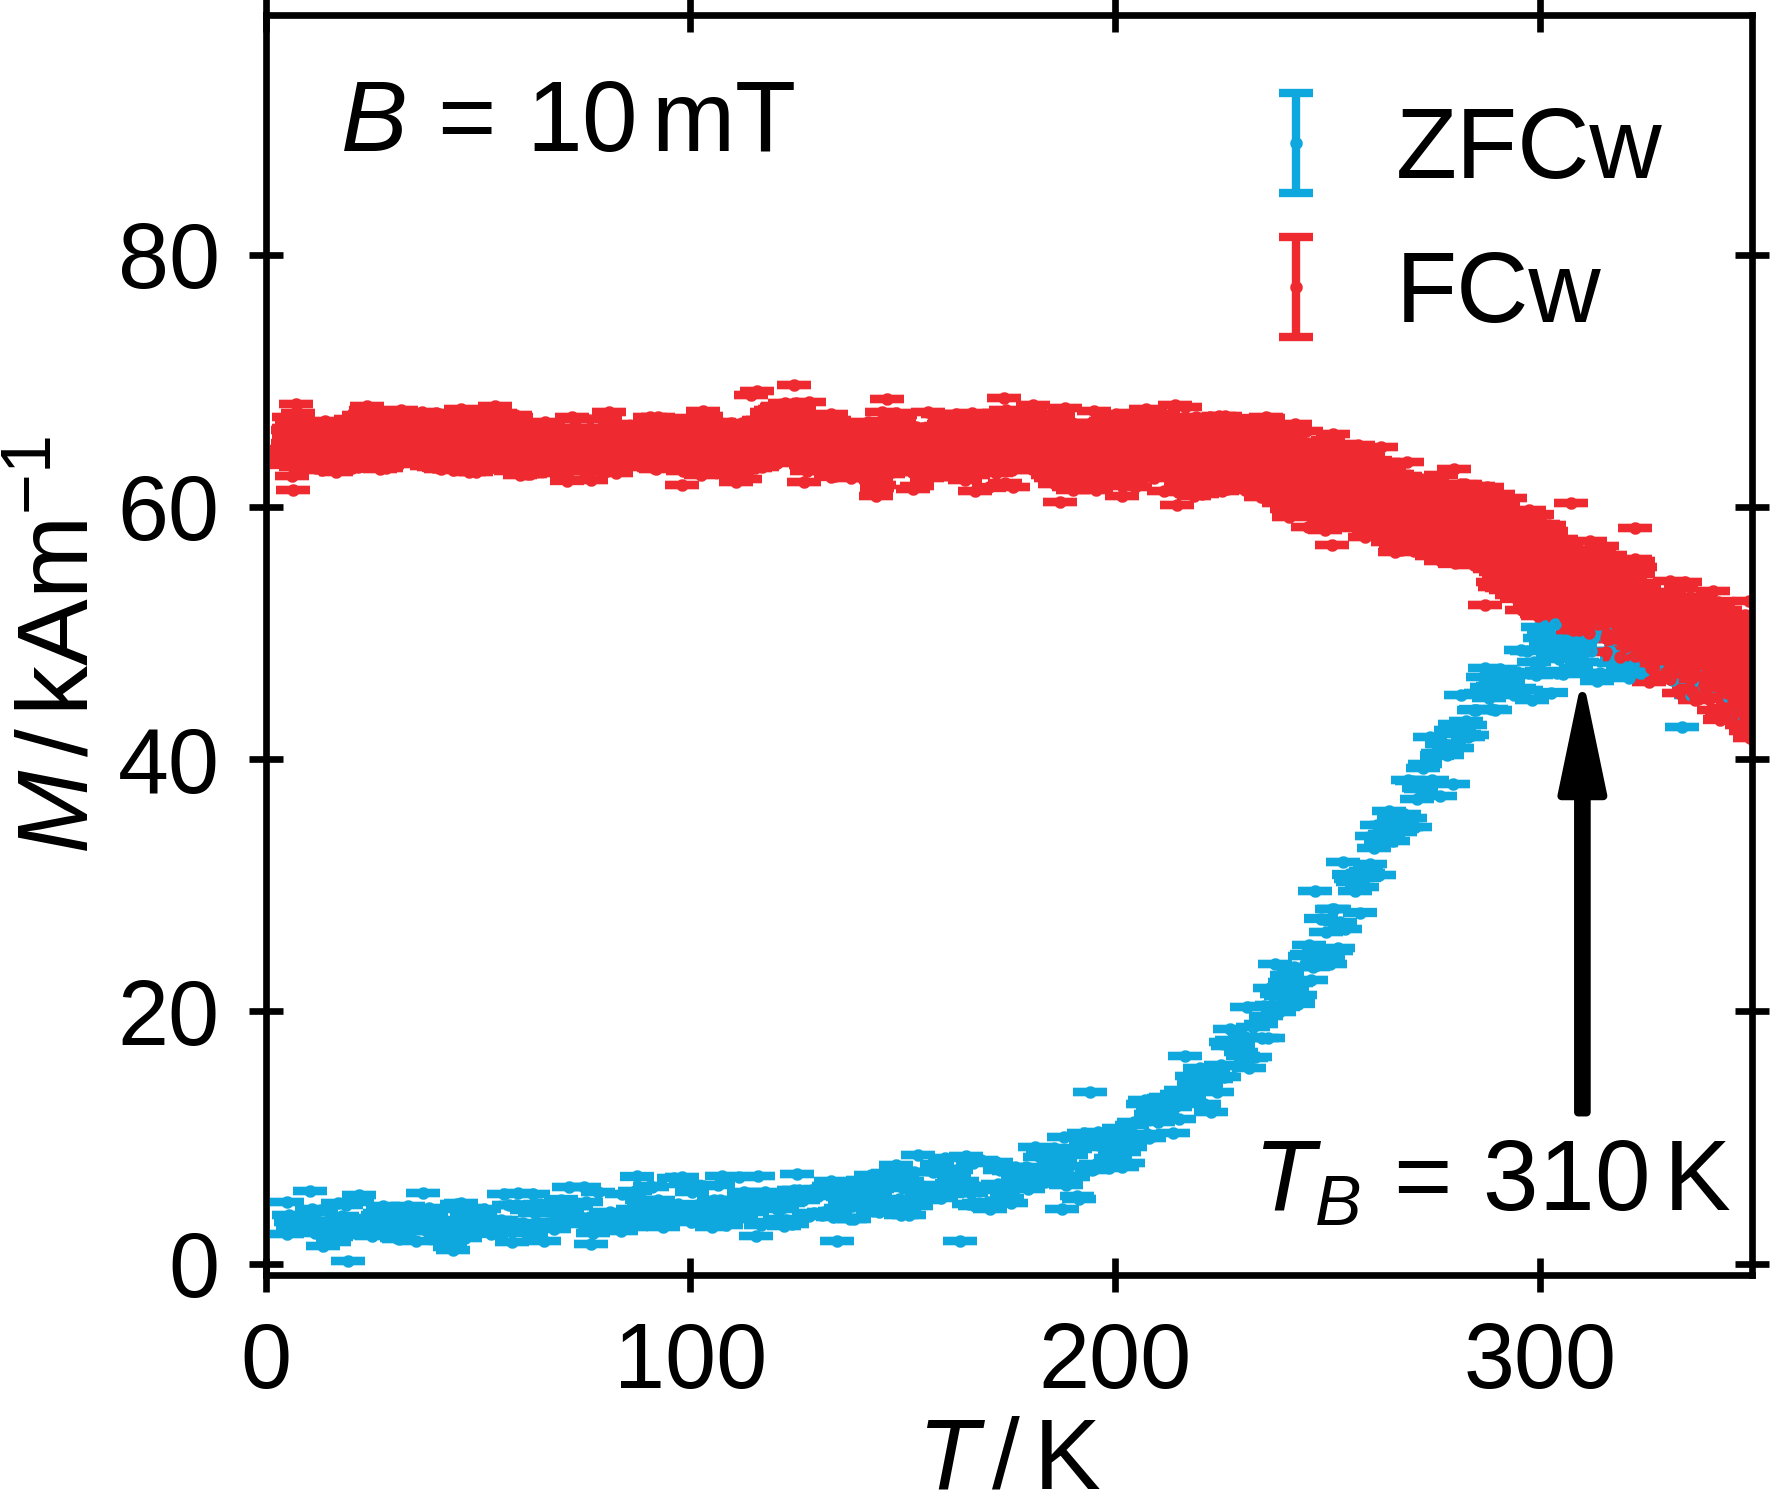
\includegraphics{monolayer_PPMS_ZFC_FC_ML_Ac_CoFe_C}
    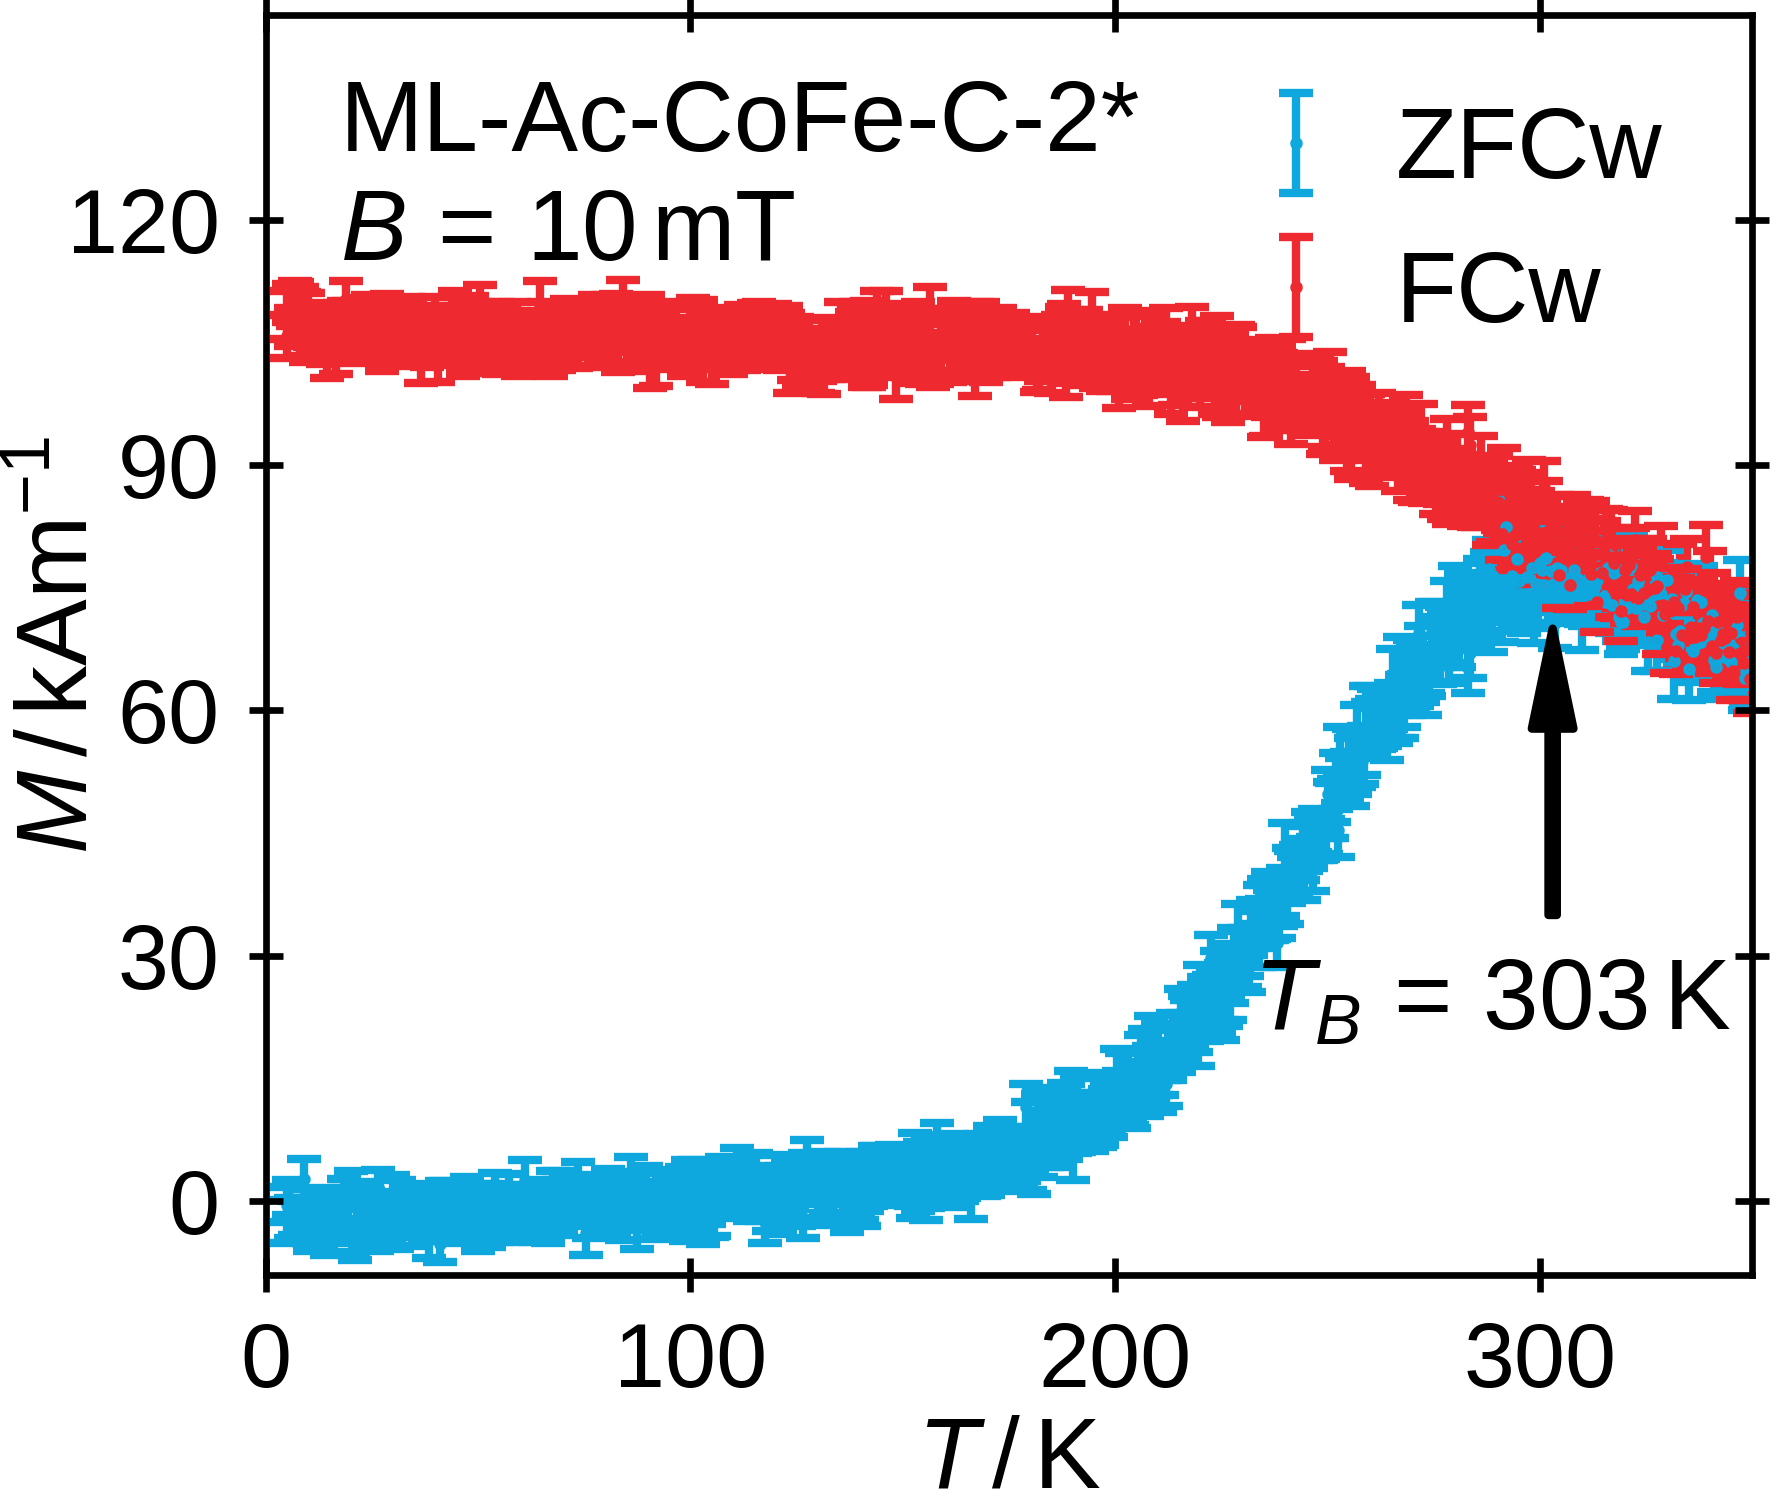
\includegraphics{monolayer_PPMS_ZFC_FC_ML_Ac_CoFe_C_2star}
    \caption{\label{fig:monolayer:magneticStructure:ppmsZFCFC}Temperature-dependent magnetization of the ordered monolayers ML-Ac-CoFe-C (left) and ML-Ac-CoFe-C-2 (right) measured at a magnetic field of $10 \unit{mT}$ during warming after zero-field and field cooling.}
  \end{figure}

  \begin{figure}[!htbp]
    \centering
    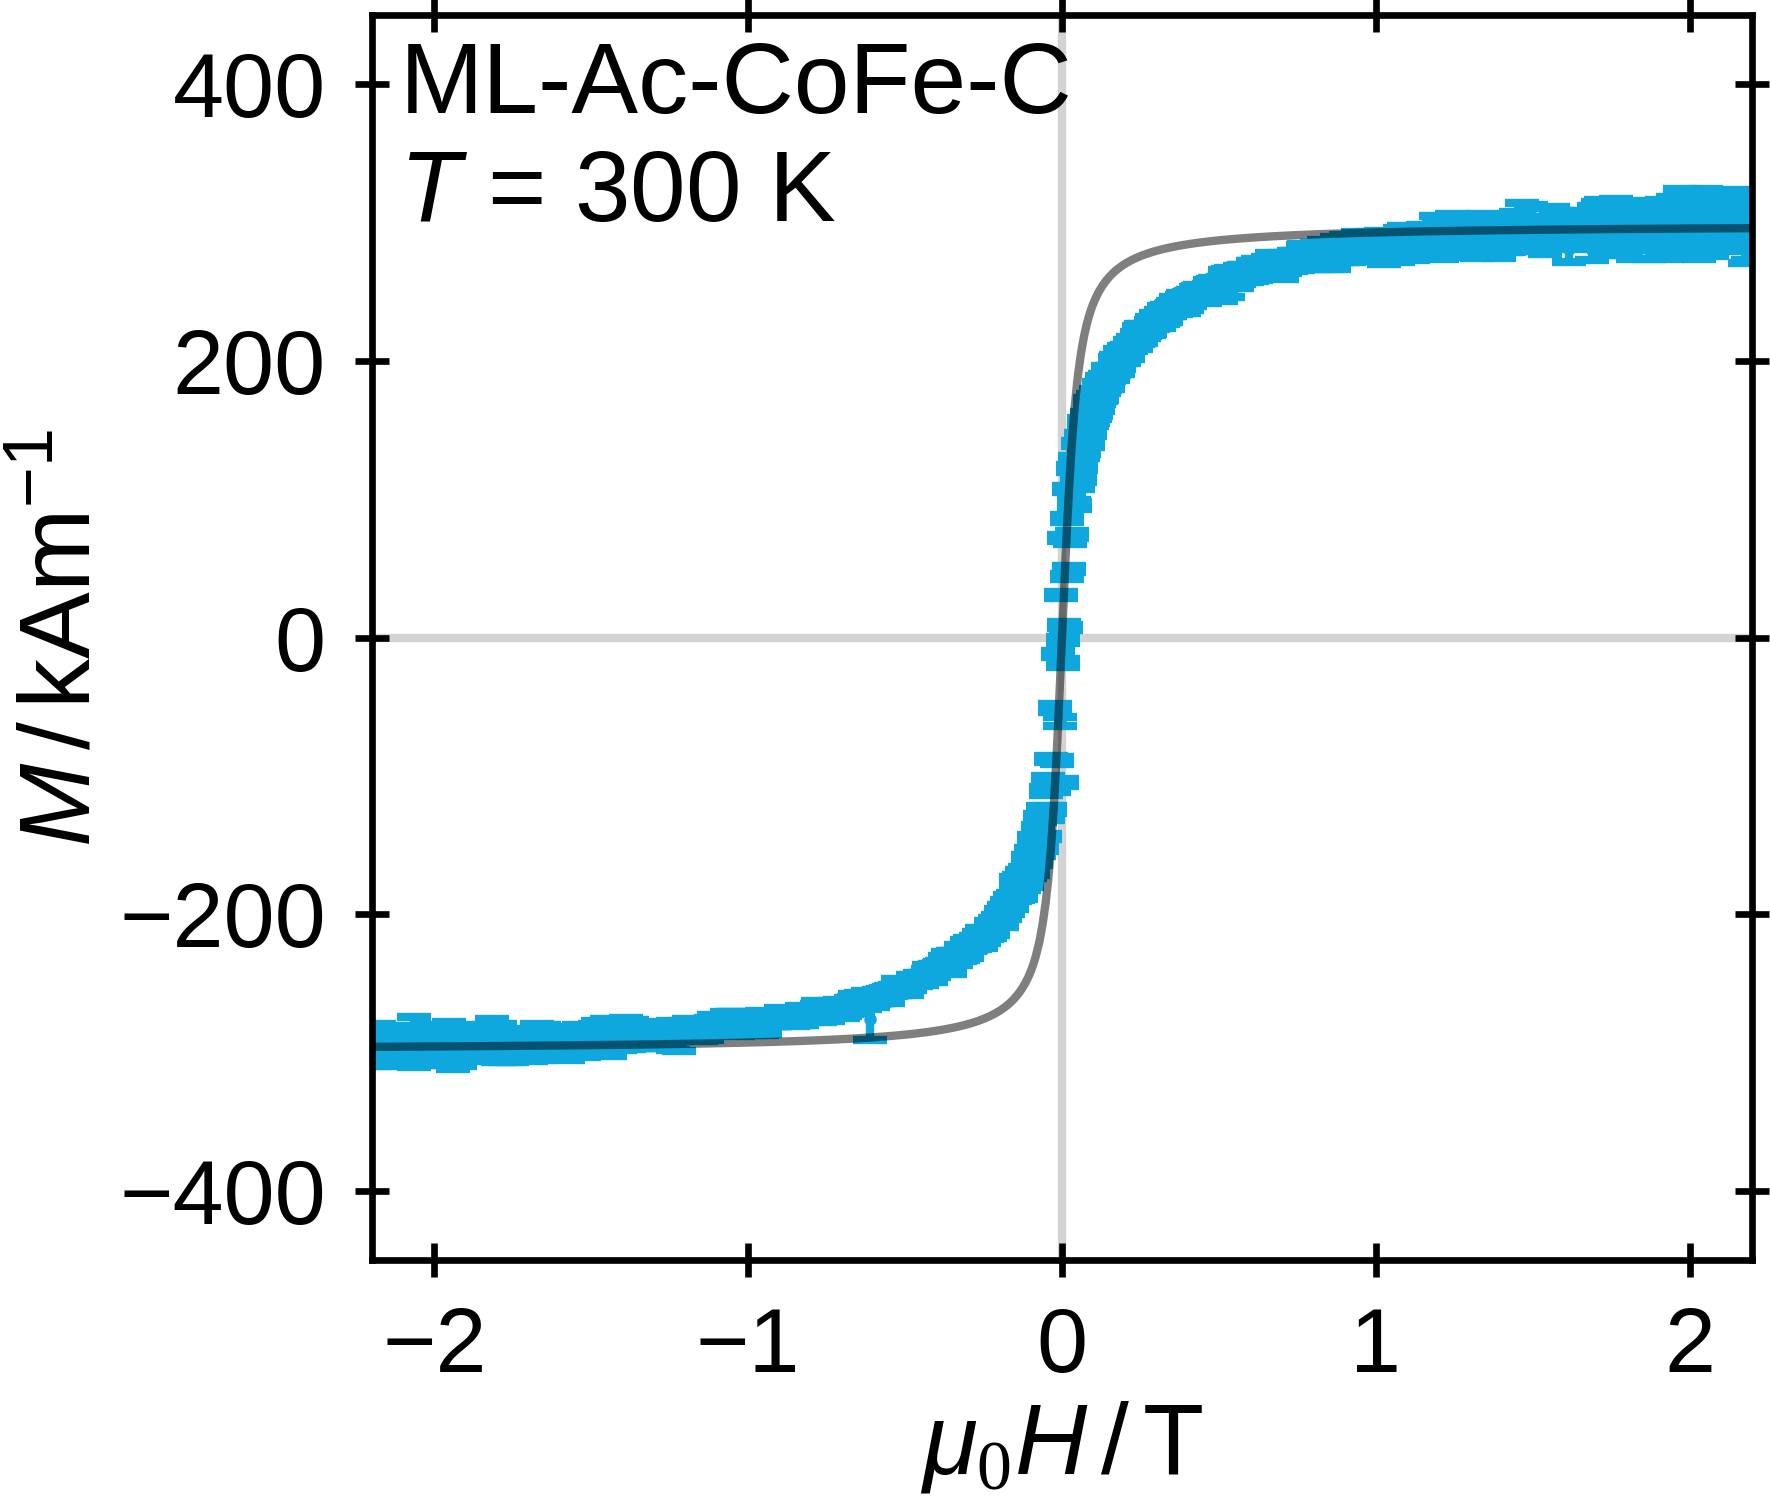
\includegraphics{monolayer_PPMS_VSM_300K_ML_Ac_CoFe_C}
    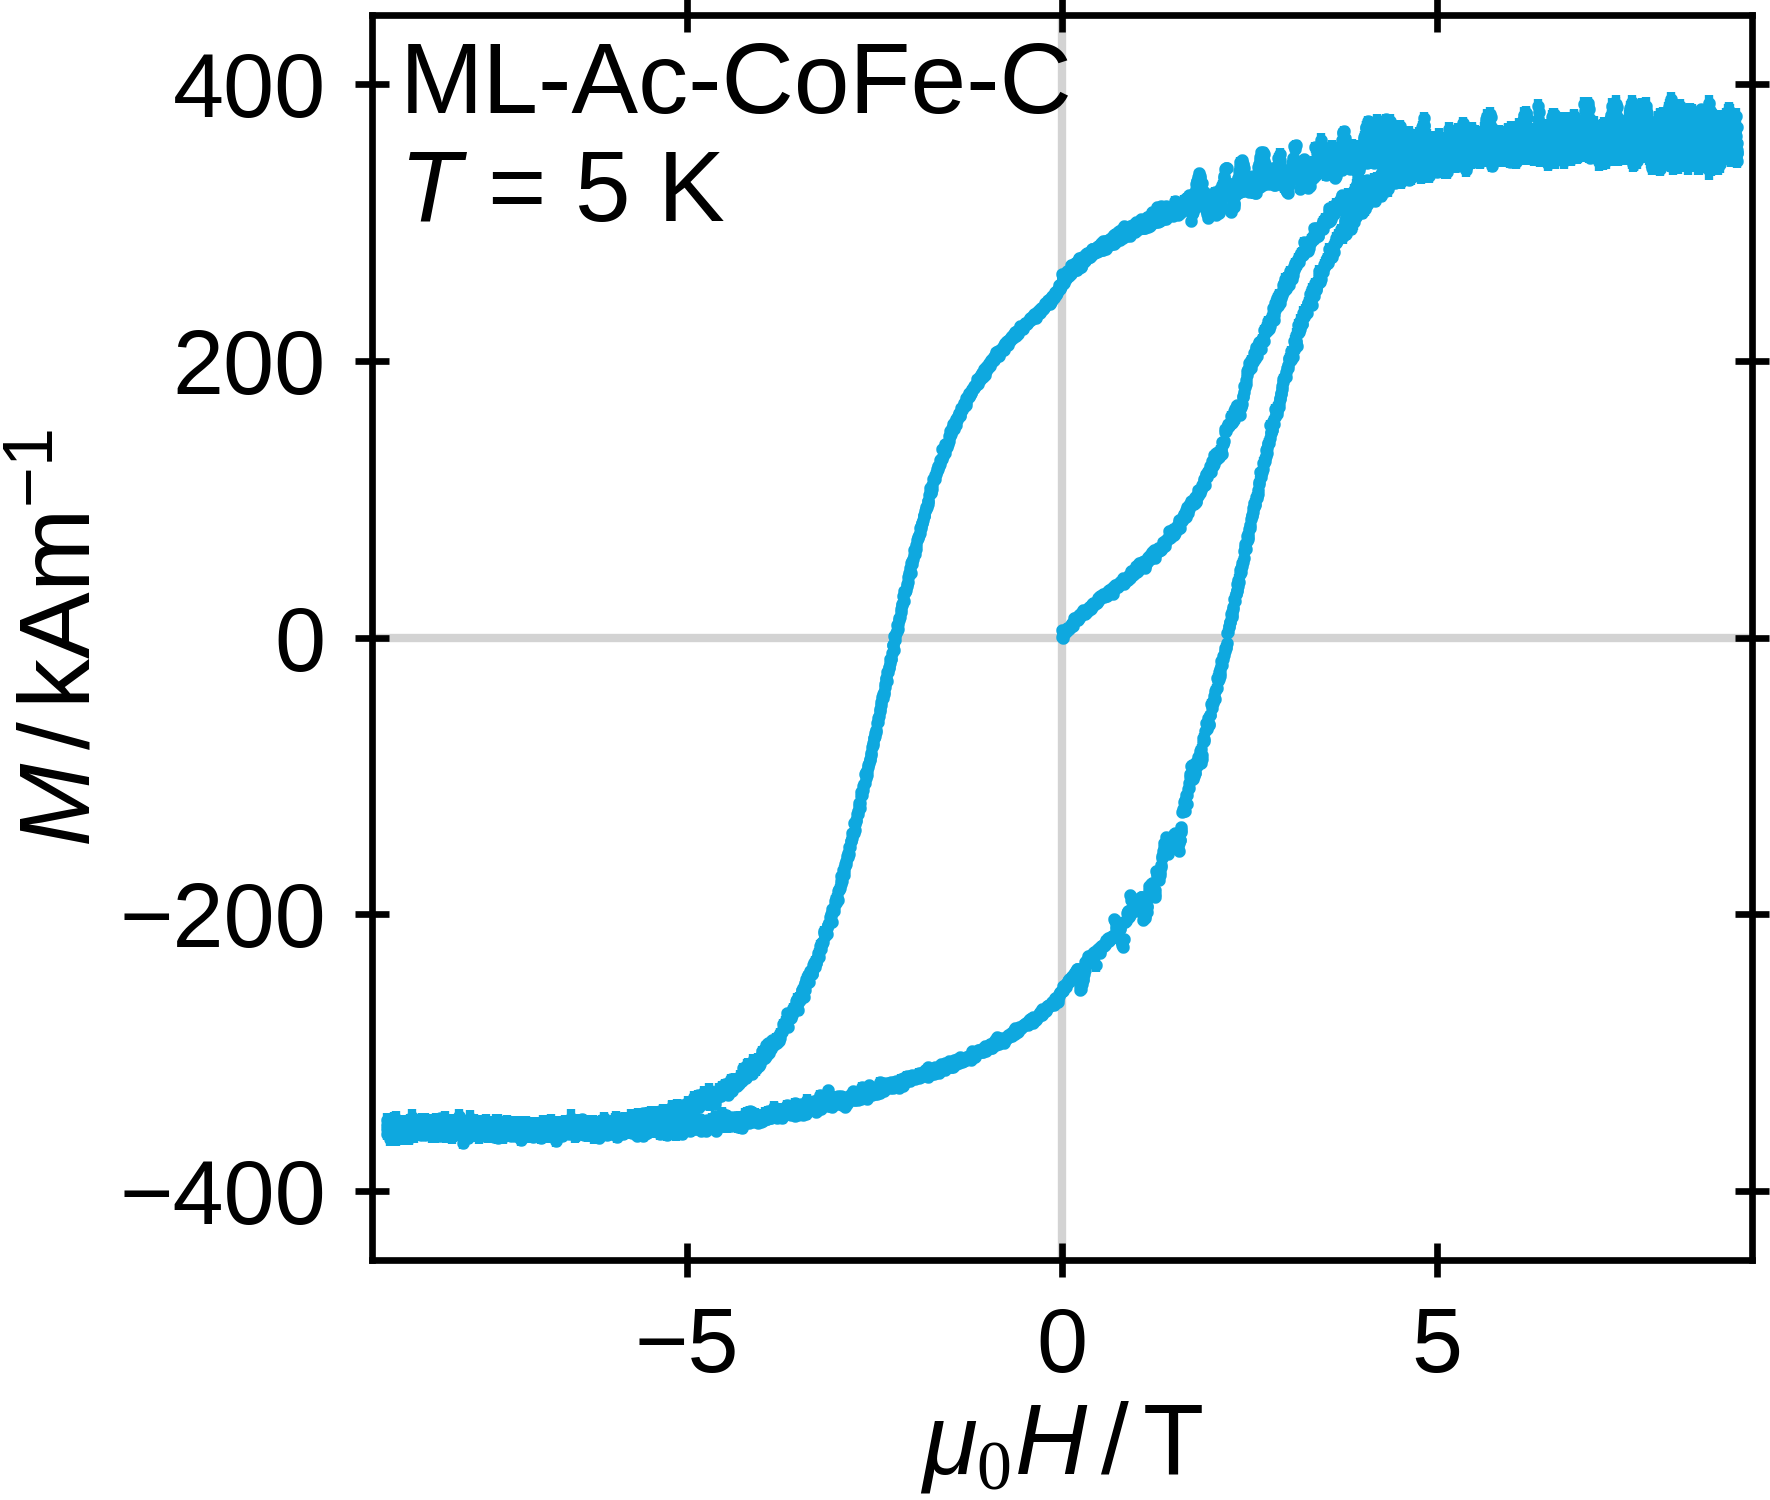
\includegraphics{monolayer_PPMS_VSM_5K_ML_Ac_CoFe_C}
    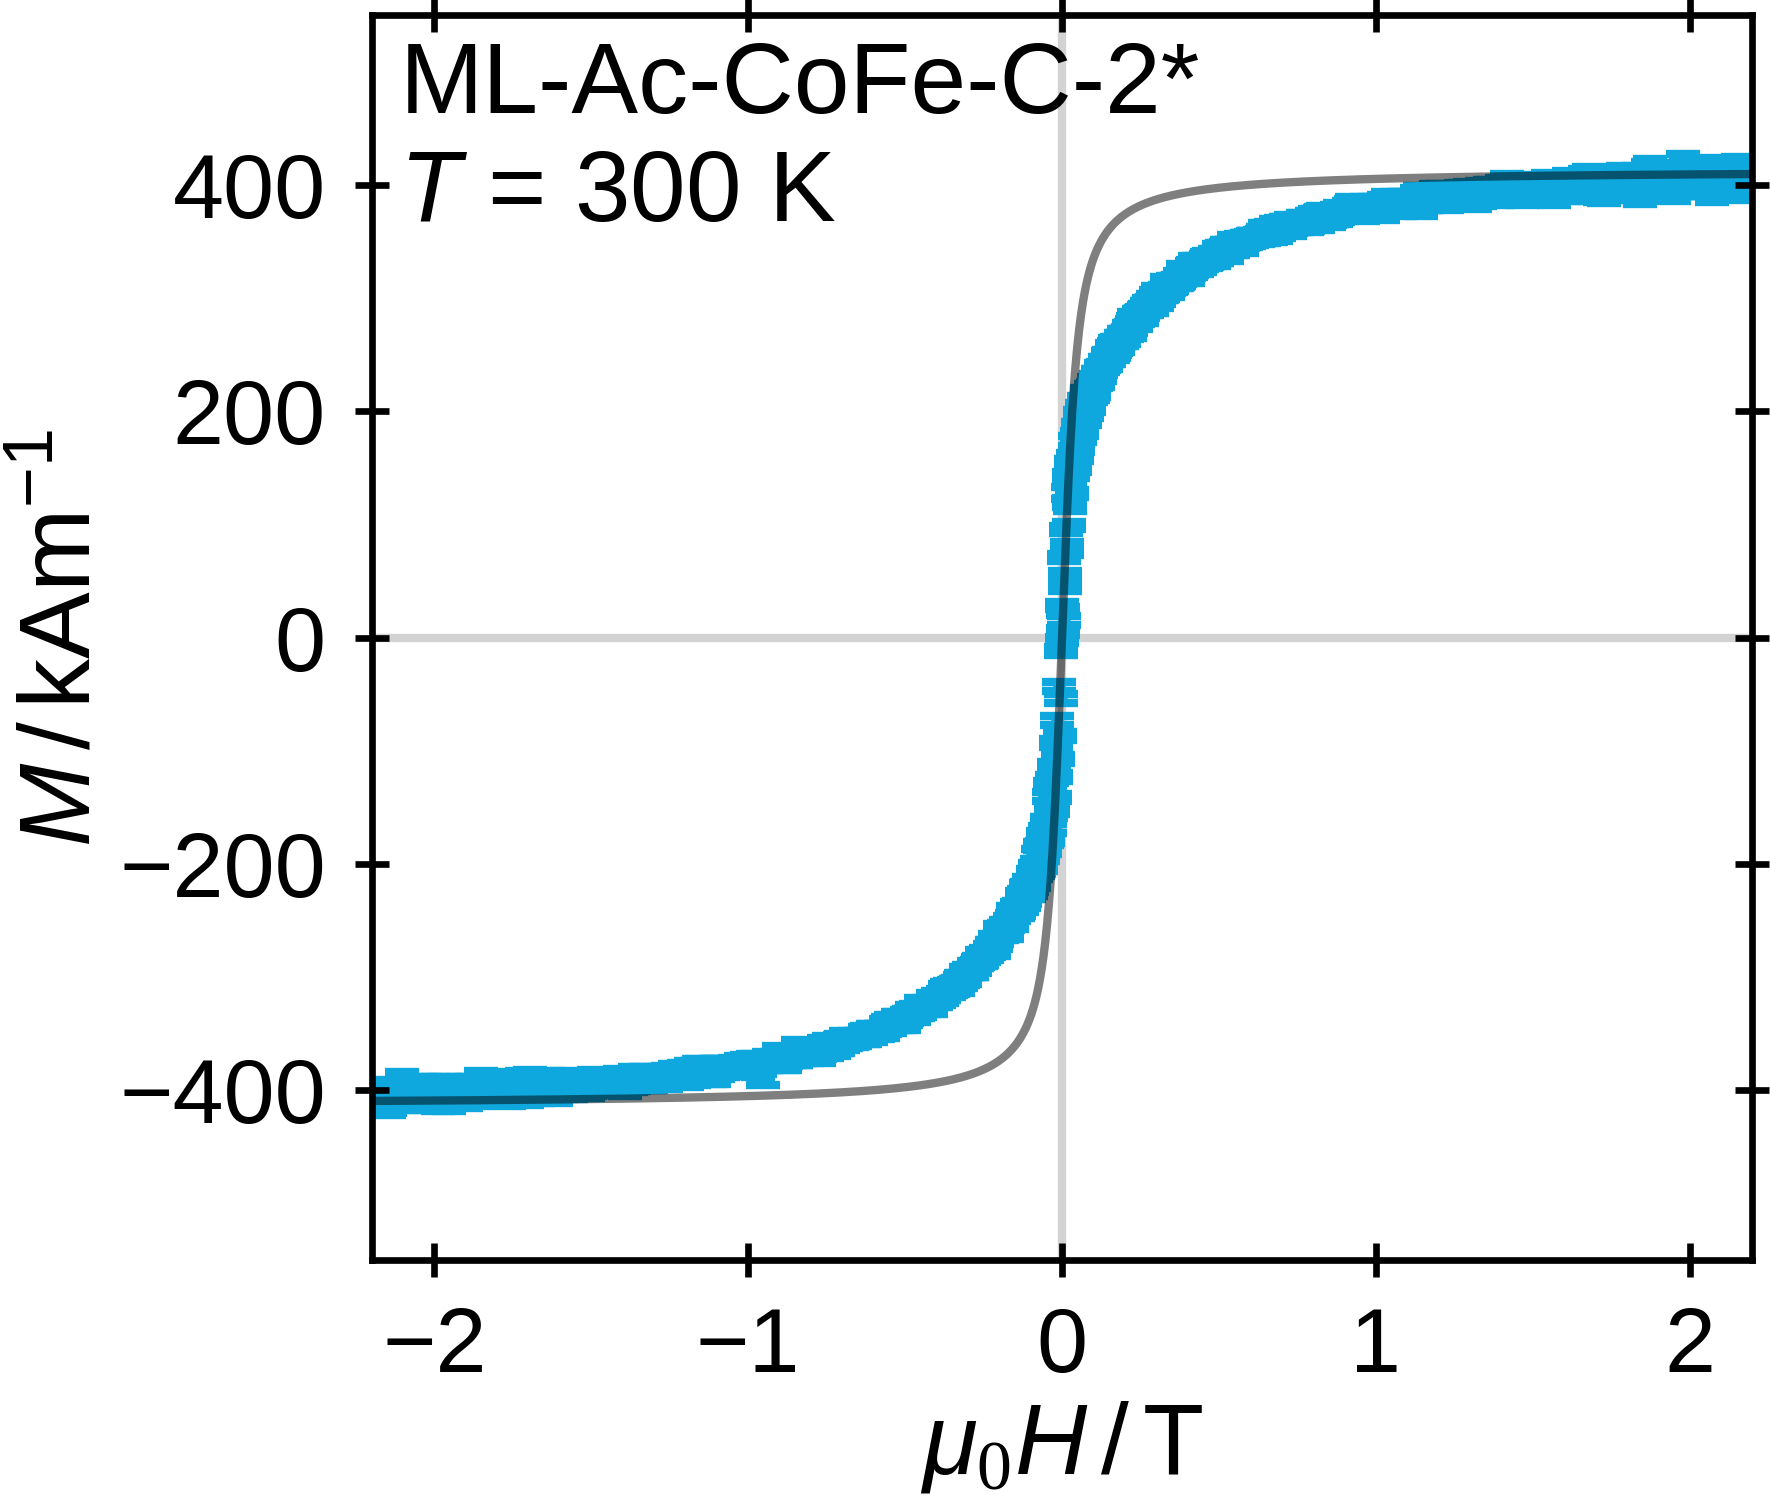
\includegraphics{monolayer_PPMS_VSM_300K_ML_Ac_CoFe_C_2star}
    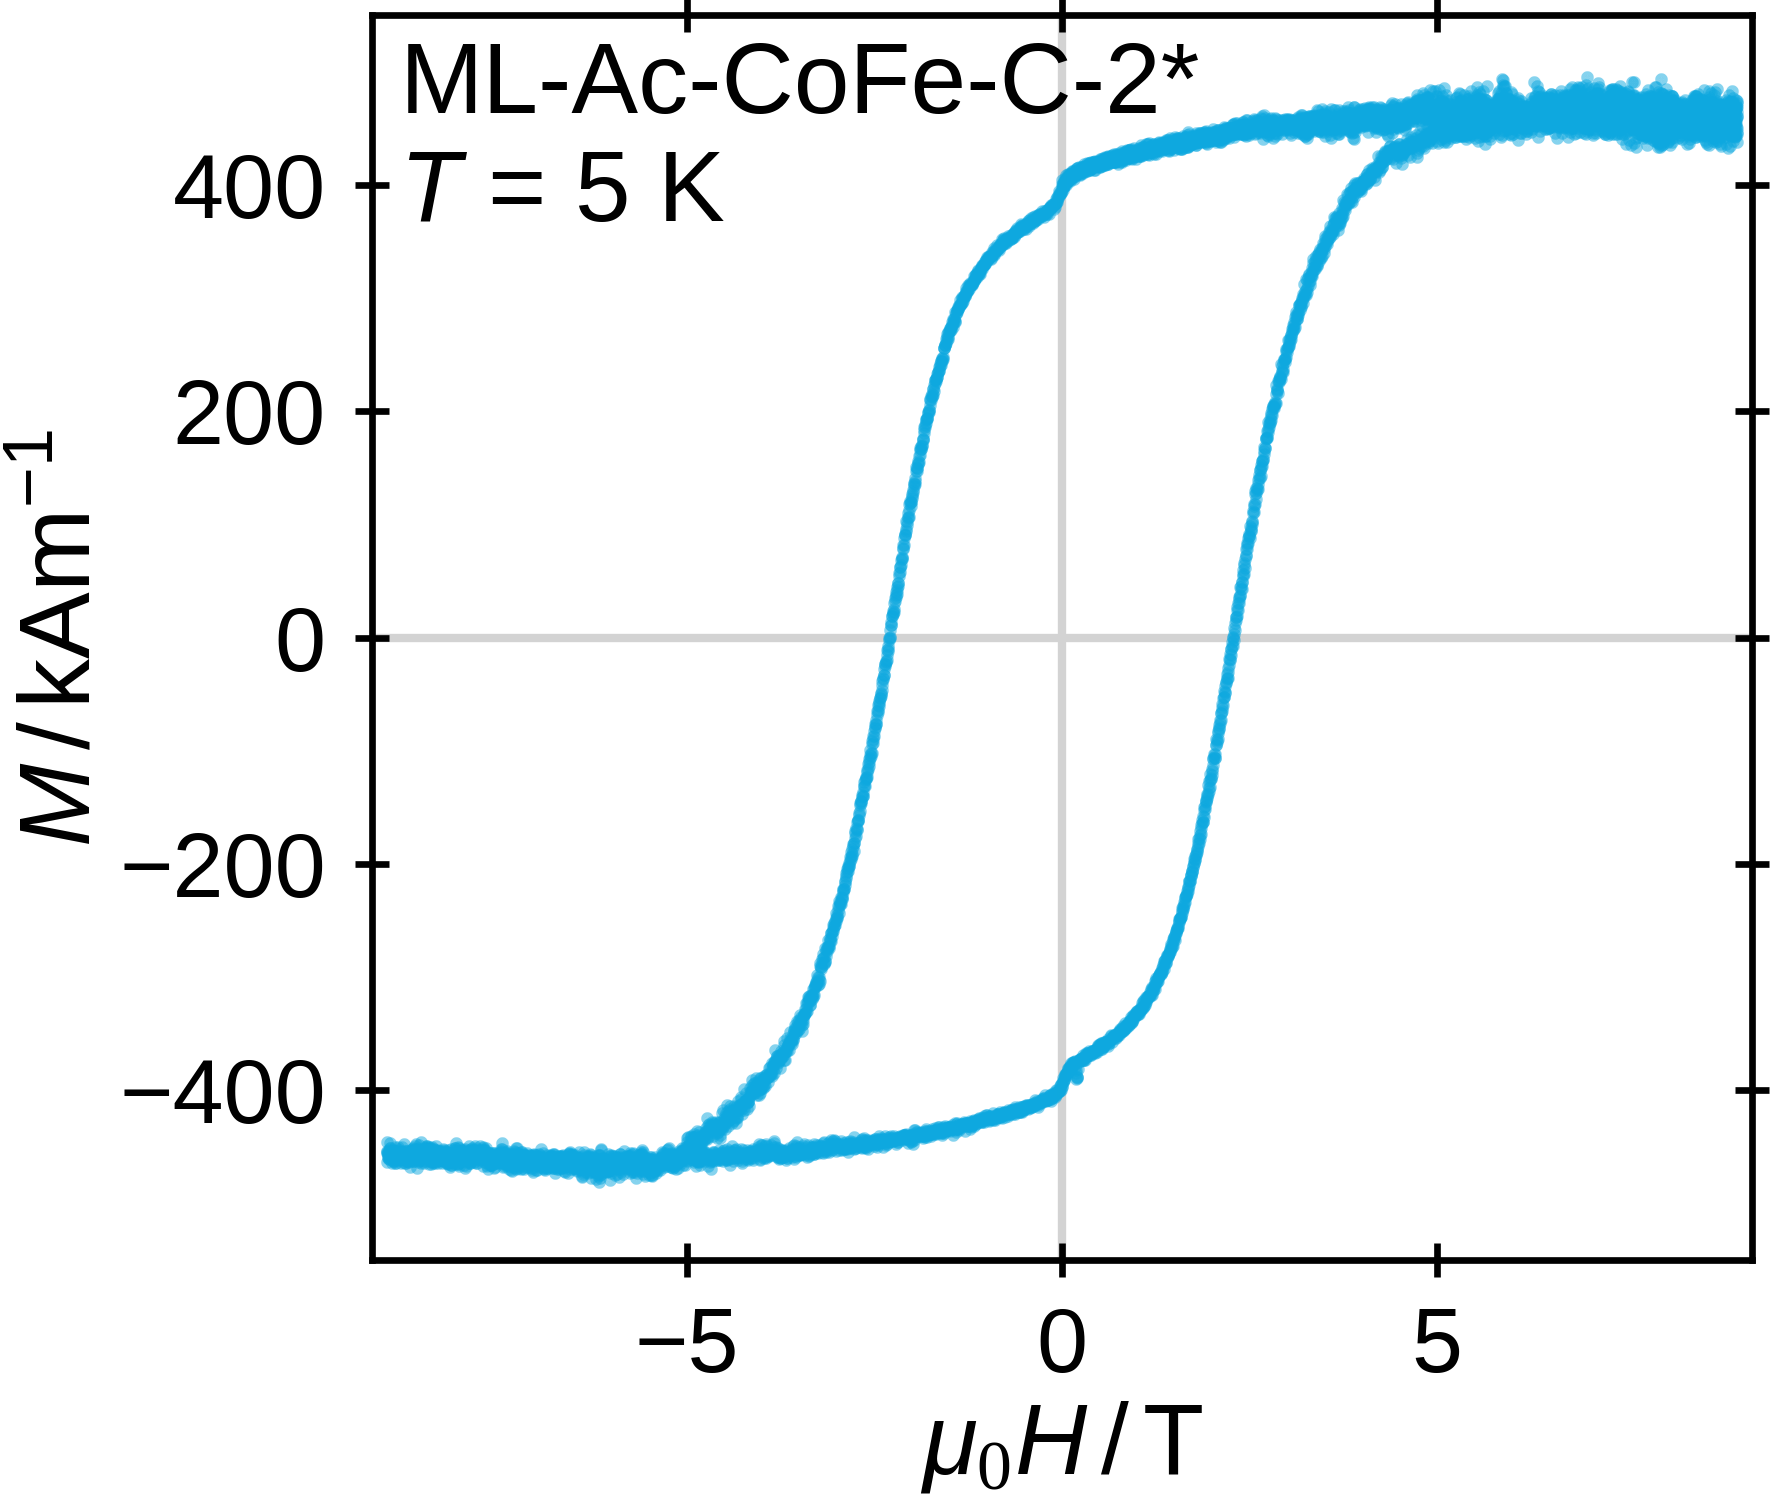
\includegraphics{monolayer_PPMS_VSM_5K_ML_Ac_CoFe_C_2star}
    \caption{\label{fig:monolayer:magneticStructure:MLAcCoFeC12}Field-dependent magnetization measurement of ML-Ac-CoFe-C (upper) and ML-Ac-CoFe-C-2* (lower) at $300 \unit{K}$ (left) and $5 \unit{K}$ (right). The Langevin magnetization of the nanocubes Ac-CoFe-C and Ac-CoFe-C-2 in dispersion at room temperature is added for direct comparison in the left plots.}
  \end{figure}

  The temperature-dependent magnetizations of the monolayers ML-Ac-CoFe-C and ML-Ac-CoFe-C-2* are shown in \reffig{fig:monolayer:magneticStructure:ppmsZFCFC}.
  ML-Ac-CoFe-C-2* is hereby an equivalently prepared sample to ML-Ac-CoFe-C-2 that is reproduced for the magnetic characterization to avoid destroying the original sample that has been used for polarized GISANS measurements.
  The blocking temperature of the monolayers is found above room temperature in both cases, with $315 \unit{K}$ observed for ML-Ac-CoFe-C and $303 \unit{K}$ for ML-Ac-CoFe-C-2*.
  Furthermore, the field cooled warming curves show a plateau at lower temperatures and no peculiar transition temperatures are visible in the measured range.

  To study the field-dependent magnetization of the monolayers ML-Ac-CoFe-C and ML-Ac-CoFe-C-2*, both monolayers were measured at $300 \unit{K}$ and $5 \unit{K}$, which is shown in \reffig{fig:monolayer:magneticStructure:MLAcCoFeC12}. Qualitatively, both monolayers show a similar magnetic behaviour.
  The room temperature measurement at $300 \unit{K}$ additionally include the Langevin behaviour that has been observed for the respective nanocubes in dispersion for direct comparison.
  The magnetization of the monolayers increases slower with respect to the externally applied field in comparison to the freely moving and non-interacting nanocubes in dispersion.
  Also a small hysteresis with a coercive field in the order of $6 \unit{mT}$ is visible on close inspection of ML-Ac-CoFe-C and in the order of $3 \unit{mT}$ for ML-Ac-CoFe-C-2*.
  This connects to the temperature-dependent magnetization measurements, which indicate that the nanocubes are close below the blocking temperature at $300 \unit{K}$.

  At the low temperature of $5 \unit{K}$, a large hysteresis is observed in both cases.
  ML-Ac-CoFe-C shows a coercive field of $2.21(1) \unit{T}$ at $5 \unit{K}$ and ML-Ac-CoFe-C-2* has a coercive field of $2.29(1) \unit{T}$.
  At small fields around $0 \unit{T}$, a jump is visible in the hysteresis in the range of $\pm 0.1 \unit{T}$, where the magnetization reduces/increases partly quicker after switching of the magnetic field direction.

  \begin{figure}[tb]
    \centering
    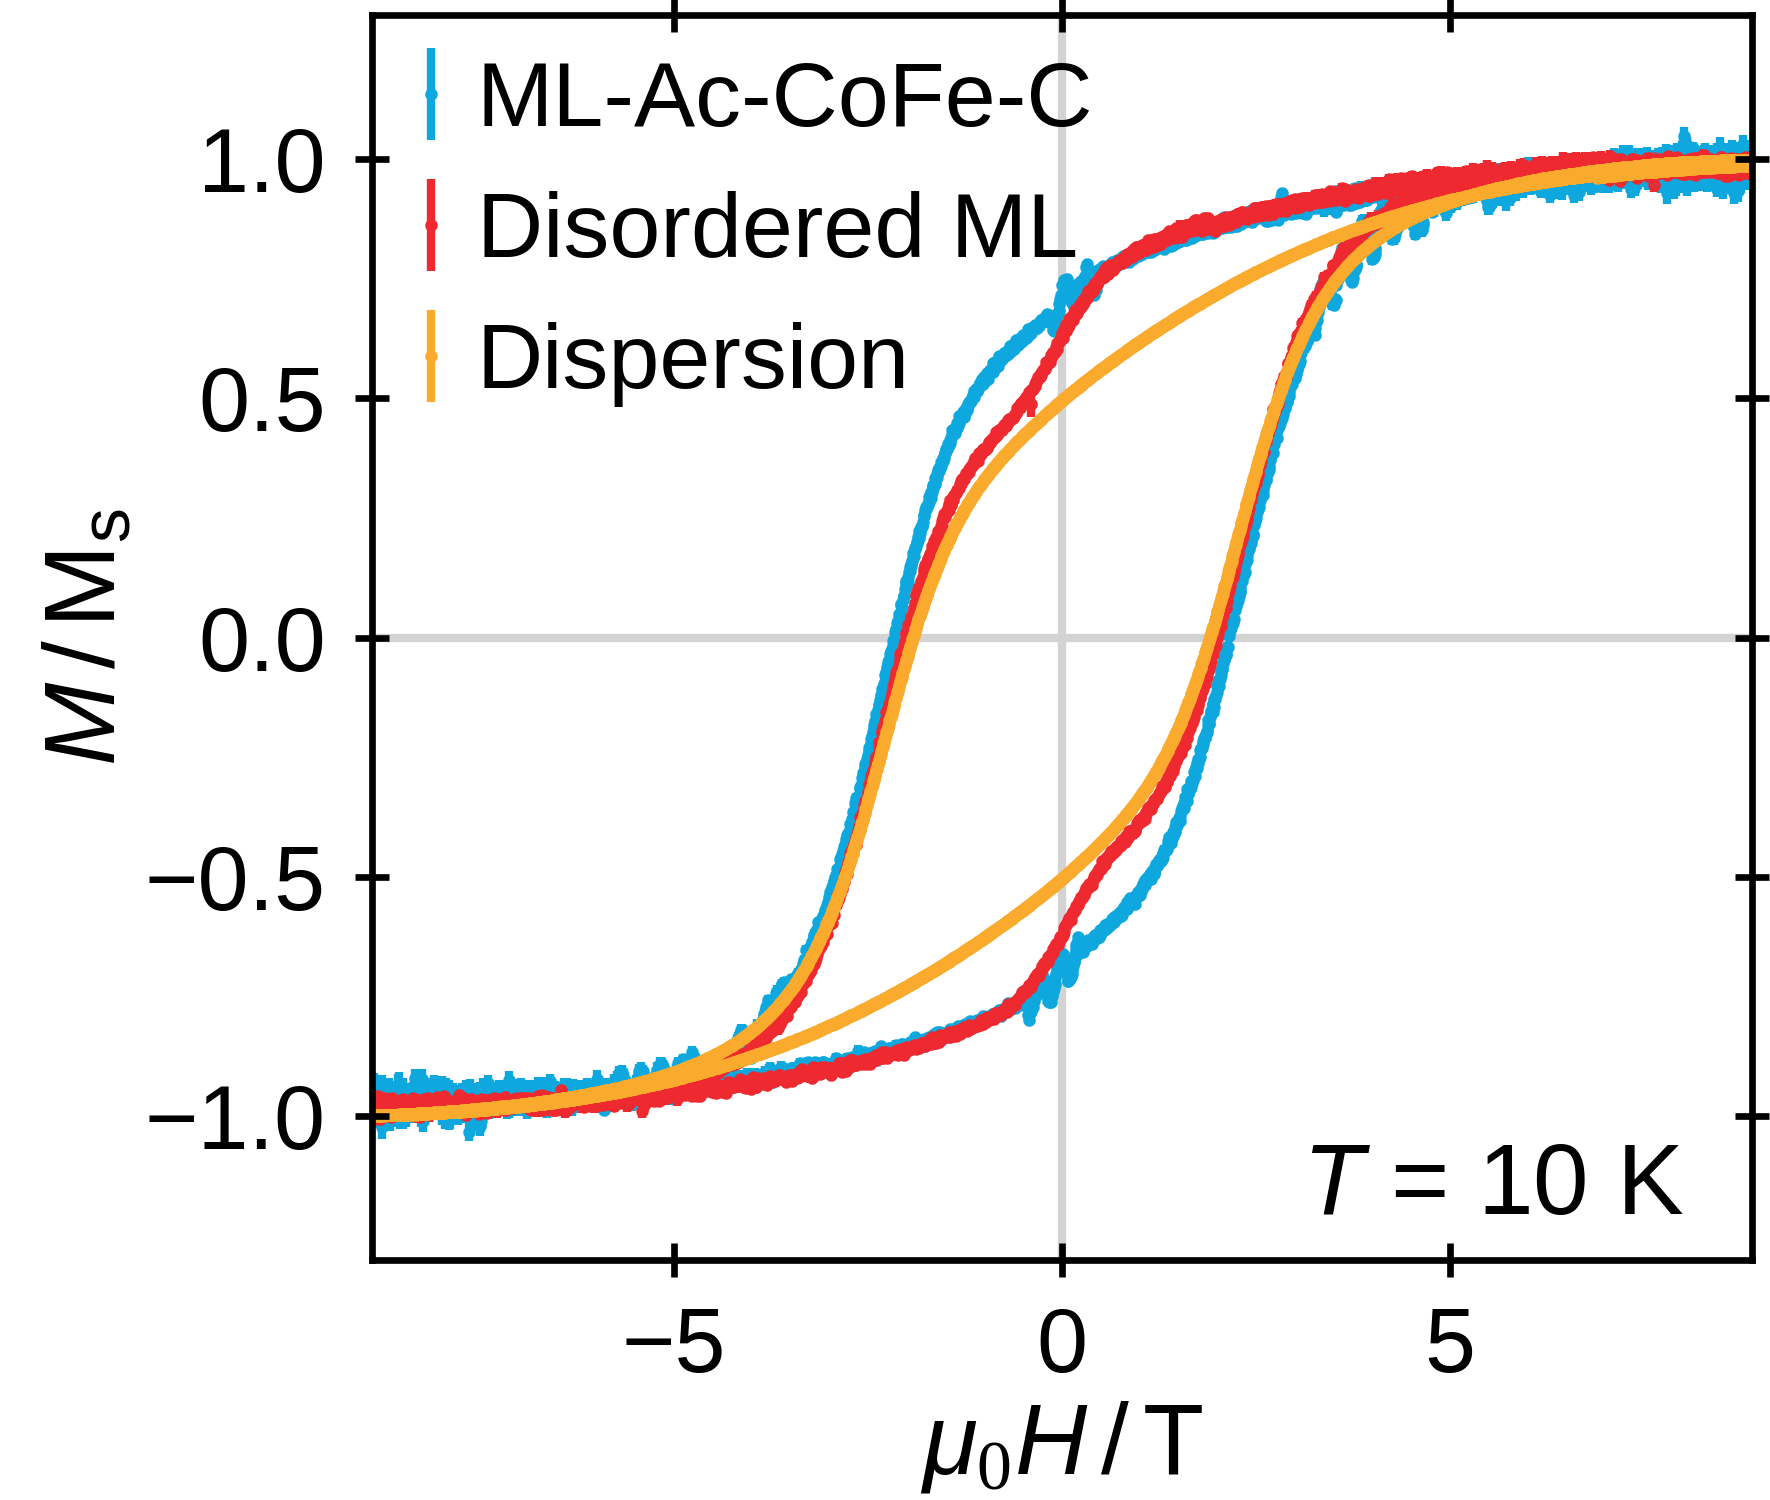
\includegraphics{monolayer_PPMS_VSM_10KCompareDispersion_ML_Ac_CoFe_C}
    \caption{\label{fig:monolayer:magneticStructure:MLAcCoFeCCompareDispWafer}Comparison of the hysteresis behaviour of Ac-CoFe-C nanocubes at $10 \unit{K}$ measured in the monolayer ML-Ac-CoFe-C, in a layer without long-range order and in dispersion.}
  \end{figure}

  To discuss the coercive field and jump in a context, the hysteresis is compared to the low-temperature magnetization of the nanocubes in a non long-range ordered state.
  In \reffig{fig:monolayer:magneticStructure:MLAcCoFeCCompareDispWafer}, the hysteretic behaviour of the monolayer ML-Ac-CoFe-C is compared to the results observed in dispersion and to the nanocubes that are dried on a wafer but without efforts to achieve long-range order, which have been also discussed in \refsec{sec:monolayers:nanoparticle:vsm}.
  As the latter two measurements were performed at $10 \unit{K}$, the shown monolayer magnetization was also measured at $10 \unit{K}$ for direct comparability.
  It is visible that the coercive field for the long-range ordered monolayer is enlarged and that the magnetization tends to decrease slower at application of a reversing magnetic field.
  For the disordered sample, it was argued that the jump in magnetization at low magnitude magnetic fields is an effect from dipolar interaction of disordered cobalt ferrite nanoparticles \cite{Alves_2017_Waspw}.
  As especially between the monolayer sample and the disordered monolayer the only difference is the long-ranged square array lattice order, the direct comparison suggests that the magnetization is stabilized by the long-range order in the monolayer, as to why stronger magnetic fields are necessary to flip once aligned domains in the sample.
  This is in contrast to the expectation for a super antiferromagnetic state, where at zero field a zero magnetization should be measured, and therefore the drop should become even stronger.
  Instead, the results can be interpret as that from the oriented state induced at the saturating field a majority is stabilized in a super ferromagnetically coupled state and therefore the coercivity is enhanced and the magnetization stabilized for reversing magnetic fields.
  % An alternative interpretation, however, can also be that in the disordered layer the nanocubes are not aligned with their (100) face relative to the substrate and the observed effect is a result from a preferred magnetocrystalline orientation of the individual nanocubes in the monolayer.
  % As VSM allows only to probe the macroscopic state, it is difficult to differentiate between the two interpretations and further information on the sample states is therefore obtained in the following by polarized neutron scattering experiments.
\end{document}